%Nous avons utilisé Git dès le début du projet, sachant qu'en plus c'est l'un des gestionnaires de version le plus performant son utilisation était évidente.
Afin de permettre une meilleure gestion du projet (travail parallèle, gestion de bugs, etc.) nous avons décidé d'utiliser le gestionnaire de version Git ainsi que la forge GitLab mise à la disposition des étudiants par le SIF.
La prise en main fut facile, les membres du groupe ayant tous déjà utilisé cet outil. Nous avons également utilisé le système de suivi de bugs intégré à Gitlab (cf. Figure~\ref{bugs}).

\begin{figure}[h]
\centering
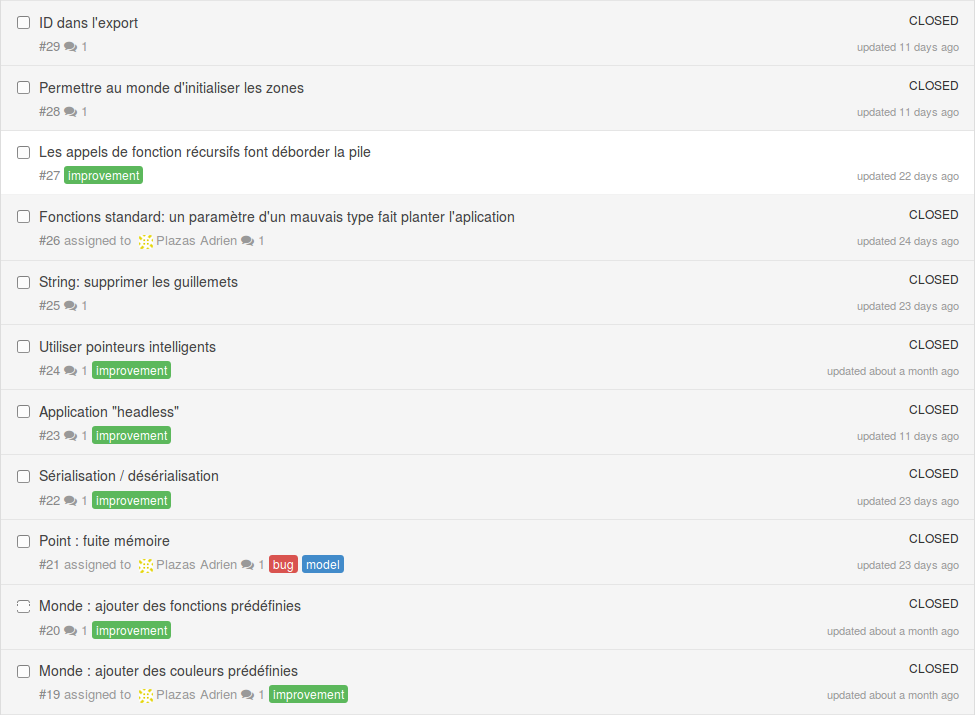
\includegraphics[scale=0.35]{doc/gestionProjet/bugs.png}
\caption{\label{bugs} Système de suivi de bugs de Gitlab}
\end{figure}

%Git permet de travailler séparement sans soucis. La prise en main s'est faite assez facilement car nous connaissions déjà cet outil, cela nous a donc permis d'en faire une utilisation plus poussée pour en avoir une meilleure gestion (utilisation de branches, des issues, etc.).
%Nous avons installé un dépôt sur le GitLab du Sif, service

%Nous avons utilisé une branche Master, qui devait contenir uniquement du code compilable, et après, chaque fonctionnalité a été développé sur une branche différente.

Notre organisation des branches fut la suivante~:
\begin{itemize}
\item la branche master devait contenir une version fontionnelle compilable~;
\item des branches de développement étaient créées pour chaque nouvelle fonctionnalité, et n'étaient fusionnées sur la branche master que lorsqu'elles étaient pleinement fonctionnelles~;
\item des branches spécifiques à chaque version ont été dérivées de master lors de l'officialisation desdites versions.
\end{itemize}

Nous utilisions également Gitg, pour avoir une meilleure vue de l'état de notre dépôt (cf. Figure~\ref{Gitg}).

\begin{figure}[h]
\centering
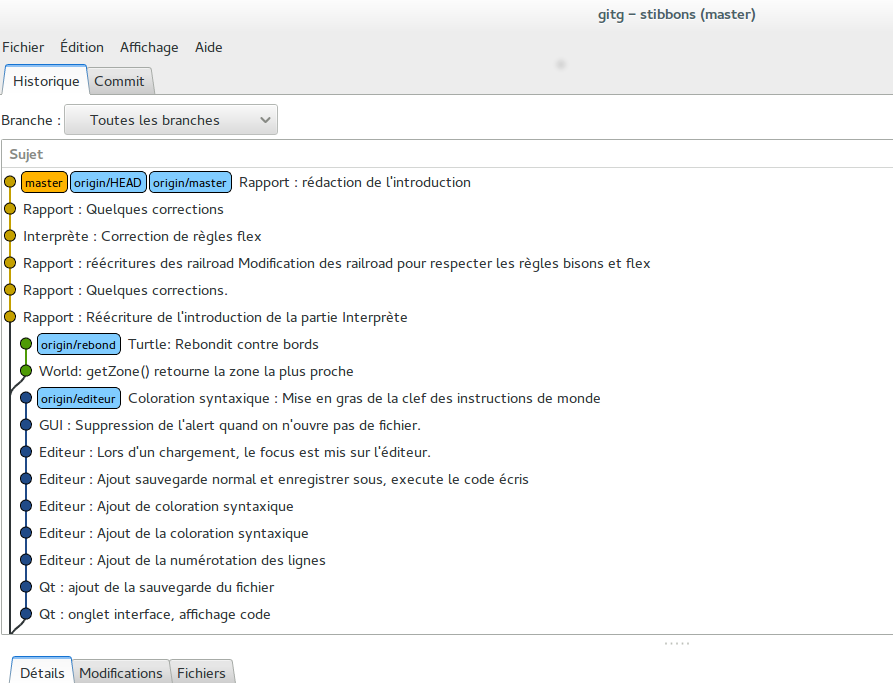
\includegraphics[scale=0.35]{doc/gestionProjet/gitbranche.png}
\caption{\label{Gitg} Vue des branches dans Gitg}
\end{figure}

% nb de ligne : wc -l `find . -name "*.h"` `find . -name "*.cpp"` `find . -name "*.y\+"` `find . -name "*.l\+"`
Lors de la sortie de la version 1.0, le dépôt comprenait 493 commits, avec une moyenne de 4,7 commits par jour, soit 98,6 commits par version en moyenne, 12 branches et aucune étiquette (nous avons utilisé les branches afin d'étiqueter les versions).
Il y avait 11~827 lignes de code réparties en 324 lignes pour l'application console, 1~496 lignes pour l'application graphique, 3~027 lignes pour l'interprète, 6~188 lignes pour le modèle et 792 lignes pour les tests.

\begin{figure}[h]
\centering
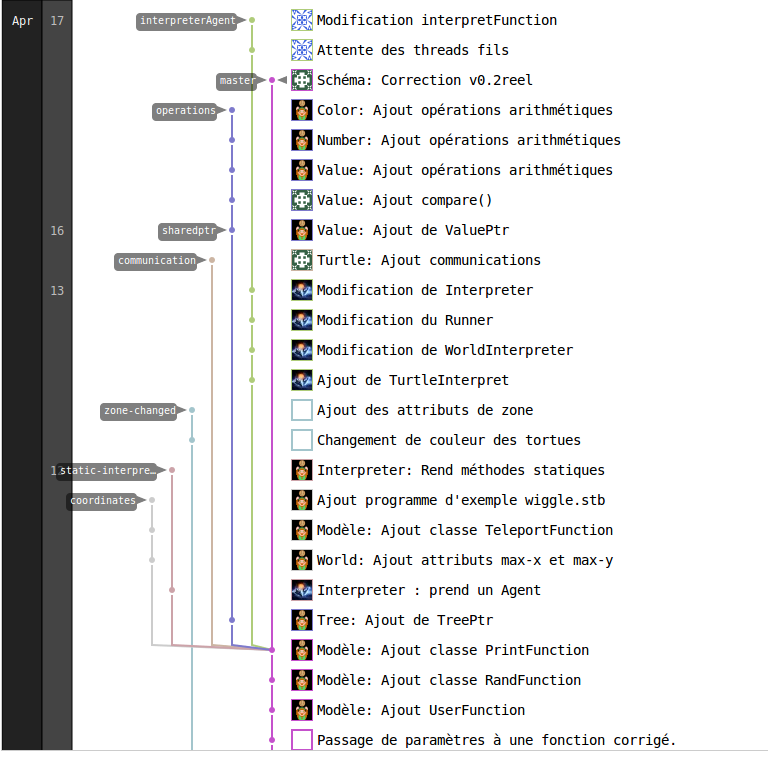
\includegraphics[scale=0.35]{doc/report/uml/network-v3.png}
\caption{\label{branche} Vue des branches lors de la version 0.3 sur Gitlab}
\end{figure}

